\subsection{Definition}
\frame{
  \frametitle{Was ist MapReduce}
}

\frame{
  \frametitle{Google Matrix / Page Rank}
\begin{center}
\only<1>{
  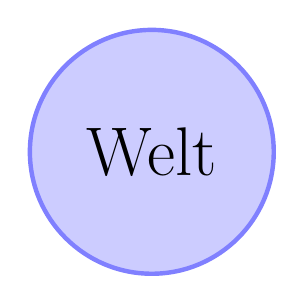
\begin{tikzpicture}
  \node[circle,fill=blue!20,draw=blue!50,ultra thick,inner sep=.5cm] {\Huge{Welt}};
\end{tikzpicture}}

\only<2>{
    %\column{.5\textwidth}
  \begin{tikzpicture}
  \node[circle,fill=blue!20,draw=blue!50,ultra thick,text width=1.5cm,align=center] (northAmerica) {Nord Amerika};
  \node[circle,fill=blue!20,draw=blue!50,ultra thick,text width=1.5cm,align=center] (southAmerica)[below=1mm of northAmerica] {Süd Amerika};
  \node[circle,fill=blue!20,draw=blue!50,ultra thick] (Europa) [right=1cm of northAmerica] {Europa};
  \node[circle,fill=blue!20,draw=blue!50,ultra thick] (Afrika)[below=5mm of Europa] {Afrika};
  \node[circle,fill=blue!20,draw=blue!50,ultra thick] (Asien) [right=1mm of Europa] {Asien};
  \node[circle,fill=blue!20,draw=blue!50,ultra thick] (Australien) [right=1cm of Afrika,yshift=-5mm] {Australien};
\end{tikzpicture}
}
\end{center}
}

\frame{
  \frametitle{Funktionierender Algorithmus}
\begin{center}
  \begin{tikzpicture}
  %\node[rectangle,fill=blue!20,draw=blue!50,ultra thick,align=center] (matrix) {pseudo Google Matrix generieren};
  %\node[rectangle,fill=red!20,draw=red!50,thick](TotMatrix)[below=1cm of matrix, xshift=-3cm]{};
  %\node[->,shape=arc,180:30:1cm,thick]()[below=1cm of matrix, xshift=-3cm]{all in one};
  \node[rectangle,fill=blue!20,draw=blue!50,ultra thick,align=center] (matrix) {pseudo Google Matrix generieren};
  \draw[->,>=stealth'](0,0) arc (0:30:3cm);
\end{tikzpicture}
\end{center}
}


%%% Local Variables: 
%%% mode: latex
%%% TeX-master: "main"
%%% End: 
